\documentclass[12pt]{article}
\usepackage[margin=2.5cm]{geometry}
\usepackage{enumerate}
\usepackage{amsfonts}
\usepackage{amsmath}
\usepackage{fancyhdr}
\usepackage{amsmath}
\usepackage{amssymb}
\usepackage{amsthm}
\usepackage{mdframed}
\usepackage{graphicx}
\usepackage{subcaption}
\usepackage{adjustbox}
\usepackage{listings}
\usepackage{xcolor}
\usepackage{booktabs}
\usepackage[utf]{kotex}

\definecolor{codegreen}{rgb}{0,0.6,0}
\definecolor{codegray}{rgb}{0.5,0.5,0.5}
\definecolor{codepurple}{rgb}{0.58,0,0.82}
\definecolor{backcolour}{rgb}{0.95,0.95,0.92}

\lstdefinestyle{mystyle}{
    backgroundcolor=\color{backcolour},
    commentstyle=\color{codegreen},
    keywordstyle=\color{magenta},
    numberstyle=\tiny\color{codegray},
    stringstyle=\color{codepurple},
    basicstyle=\ttfamily\footnotesize,
    breakatwhitespace=false,
    breaklines=true,
    captionpos=b,
    keepspaces=true,
    numbers=left,
    numbersep=5pt,
    showspaces=false,
    showstringspaces=false,
    showtabs=false,
    tabsize=1
}

\lstset{style=mystyle}

\pagestyle{fancy}
\renewcommand{\headrulewidth}{0.4pt}
\lhead{Hyungmo Gu}
\rhead{CSC209 Week 10 Notes}

\begin{document}
\title{CSC209 Week 10 Notes}
\author{Hyungmo Gu}
\maketitle

\section*{C Pre-Processor 1 of 1}

\bigskip

\begin{itemize}
    \item Macros
    \begin{itemize}
        \item Starts with `\# define'
        \item Can also be an expression with parameters

    \begin{lstlisting}[language=c]
    #define WITH_TAX(x) ((x) * 1.08) //<- NOTE: there is no space between WITH_TAX and (x)
    \end{lstlisting}

        \begin{itemize}
            \item IMPORTANT: Always surround macro variables with parenthesis
    \begin{lstlisting}[language=c, caption={macros\_example\_1.c}]
    #define WITH_TAX(x) (x * 1.08)

    int main() {
        double purchase = 9.99;
        double purchase2 = 12.49;

        printf("%f\n", WITH_TAX(purchase + purchase2)); //<- will result in purchase + purchase2 * 1.08.
    }
    \end{lstlisting}
        \end{itemize}


    \end{itemize}
\end{itemize}

\bigskip

\section*{Select 1 of 2}

\bigskip

\begin{itemize}
    \item The problem with Blocking Reads
    \begin{itemize}
        \item \textit{read} waits until a pipe is non-empty, and reads one at a time
        \item suppose there are multiple-children with \textit{write}, then there may be
        \begin{enumerate}[1.]
            \item One child with empty pipe
            \item One child with filling contents, i.e. `hello', `hi there!'
        \end{enumerate}
        \item Parent waits for empty pipe, causing blocking

        \begin{center}
        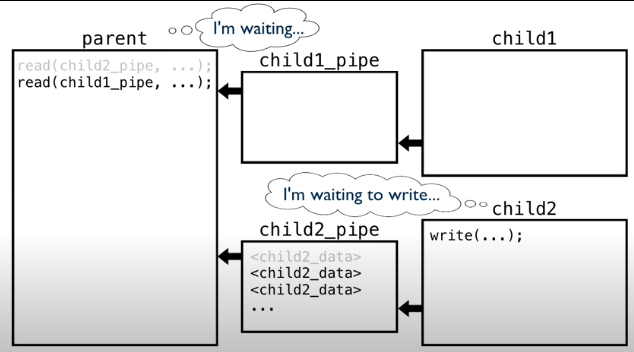
\includegraphics[width=\linewidth]{images/week_10_notes_2_1.png}
        \end{center}
        \item \textit{select} $\leftarrow$ \underline{solution}
        \begin{itemize}
            \item monitors file descriptors, waiting until one or more of the file
            descriptors become ready
        \end{itemize}
    \end{itemize}
\end{itemize}

\bigskip

\end{document}